\documentclass{article}
\usepackage{iclr2021_conference,times}

%%%%% NEW MATH DEFINITIONS %%%%%

\usepackage{amsmath,amsfonts,bm}

% Mark sections of captions for referring to divisions of figures
\newcommand{\figleft}{{\em (Left)}}
\newcommand{\figcenter}{{\em (Center)}}
\newcommand{\figright}{{\em (Right)}}
\newcommand{\figtop}{{\em (Top)}}
\newcommand{\figbottom}{{\em (Bottom)}}
\newcommand{\captiona}{{\em (a)}}
\newcommand{\captionb}{{\em (b)}}
\newcommand{\captionc}{{\em (c)}}
\newcommand{\captiond}{{\em (d)}}

% Highlight a newly defined term
\newcommand{\newterm}[1]{{\bf #1}}


% Figure reference, lower-case.
\def\figref#1{figure~\ref{#1}}
% Figure reference, capital. For start of sentence
\def\Figref#1{Figure~\ref{#1}}
\def\twofigref#1#2{figures \ref{#1} and \ref{#2}}
\def\quadfigref#1#2#3#4{figures \ref{#1}, \ref{#2}, \ref{#3} and \ref{#4}}
% Section reference, lower-case.
\def\secref#1{section~\ref{#1}}
% Section reference, capital.
\def\Secref#1{Section~\ref{#1}}
% Reference to two sections.
\def\twosecrefs#1#2{sections \ref{#1} and \ref{#2}}
% Reference to three sections.
\def\secrefs#1#2#3{sections \ref{#1}, \ref{#2} and \ref{#3}}
% Reference to an equation, lower-case.
\def\eqref#1{equation~\ref{#1}}
% Reference to an equation, upper case
\def\Eqref#1{Equation~\ref{#1}}
% A raw reference to an equation---avoid using if possible
\def\plaineqref#1{\ref{#1}}
% Reference to a chapter, lower-case.
\def\chapref#1{chapter~\ref{#1}}
% Reference to an equation, upper case.
\def\Chapref#1{Chapter~\ref{#1}}
% Reference to a range of chapters
\def\rangechapref#1#2{chapters\ref{#1}--\ref{#2}}
% Reference to an algorithm, lower-case.
\def\algref#1{algorithm~\ref{#1}}
% Reference to an algorithm, upper case.
\def\Algref#1{Algorithm~\ref{#1}}
\def\twoalgref#1#2{algorithms \ref{#1} and \ref{#2}}
\def\Twoalgref#1#2{Algorithms \ref{#1} and \ref{#2}}
% Reference to a part, lower case
\def\partref#1{part~\ref{#1}}
% Reference to a part, upper case
\def\Partref#1{Part~\ref{#1}}
\def\twopartref#1#2{parts \ref{#1} and \ref{#2}}

\def\ceil#1{\lceil #1 \rceil}
\def\floor#1{\lfloor #1 \rfloor}
\def\1{\bm{1}}
\newcommand{\train}{\mathcal{D}}
\newcommand{\valid}{\mathcal{D_{\mathrm{valid}}}}
\newcommand{\test}{\mathcal{D_{\mathrm{test}}}}

\def\eps{{\epsilon}}


% Random variables
\def\reta{{\textnormal{$\eta$}}}
\def\ra{{\textnormal{a}}}
\def\rb{{\textnormal{b}}}
\def\rc{{\textnormal{c}}}
\def\rd{{\textnormal{d}}}
\def\re{{\textnormal{e}}}
\def\rf{{\textnormal{f}}}
\def\rg{{\textnormal{g}}}
\def\rh{{\textnormal{h}}}
\def\ri{{\textnormal{i}}}
\def\rj{{\textnormal{j}}}
\def\rk{{\textnormal{k}}}
\def\rl{{\textnormal{l}}}
% rm is already a command, just don't name any random variables m
\def\rn{{\textnormal{n}}}
\def\ro{{\textnormal{o}}}
\def\rp{{\textnormal{p}}}
\def\rq{{\textnormal{q}}}
\def\rr{{\textnormal{r}}}
\def\rs{{\textnormal{s}}}
\def\rt{{\textnormal{t}}}
\def\ru{{\textnormal{u}}}
\def\rv{{\textnormal{v}}}
\def\rw{{\textnormal{w}}}
\def\rx{{\textnormal{x}}}
\def\ry{{\textnormal{y}}}
\def\rz{{\textnormal{z}}}

% Random vectors
\def\rvepsilon{{\mathbf{\epsilon}}}
\def\rvtheta{{\mathbf{\theta}}}
\def\rva{{\mathbf{a}}}
\def\rvb{{\mathbf{b}}}
\def\rvc{{\mathbf{c}}}
\def\rvd{{\mathbf{d}}}
\def\rve{{\mathbf{e}}}
\def\rvf{{\mathbf{f}}}
\def\rvg{{\mathbf{g}}}
\def\rvh{{\mathbf{h}}}
\def\rvu{{\mathbf{i}}}
\def\rvj{{\mathbf{j}}}
\def\rvk{{\mathbf{k}}}
\def\rvl{{\mathbf{l}}}
\def\rvm{{\mathbf{m}}}
\def\rvn{{\mathbf{n}}}
\def\rvo{{\mathbf{o}}}
\def\rvp{{\mathbf{p}}}
\def\rvq{{\mathbf{q}}}
\def\rvr{{\mathbf{r}}}
\def\rvs{{\mathbf{s}}}
\def\rvt{{\mathbf{t}}}
\def\rvu{{\mathbf{u}}}
\def\rvv{{\mathbf{v}}}
\def\rvw{{\mathbf{w}}}
\def\rvx{{\mathbf{x}}}
\def\rvy{{\mathbf{y}}}
\def\rvz{{\mathbf{z}}}

% Elements of random vectors
\def\erva{{\textnormal{a}}}
\def\ervb{{\textnormal{b}}}
\def\ervc{{\textnormal{c}}}
\def\ervd{{\textnormal{d}}}
\def\erve{{\textnormal{e}}}
\def\ervf{{\textnormal{f}}}
\def\ervg{{\textnormal{g}}}
\def\ervh{{\textnormal{h}}}
\def\ervi{{\textnormal{i}}}
\def\ervj{{\textnormal{j}}}
\def\ervk{{\textnormal{k}}}
\def\ervl{{\textnormal{l}}}
\def\ervm{{\textnormal{m}}}
\def\ervn{{\textnormal{n}}}
\def\ervo{{\textnormal{o}}}
\def\ervp{{\textnormal{p}}}
\def\ervq{{\textnormal{q}}}
\def\ervr{{\textnormal{r}}}
\def\ervs{{\textnormal{s}}}
\def\ervt{{\textnormal{t}}}
\def\ervu{{\textnormal{u}}}
\def\ervv{{\textnormal{v}}}
\def\ervw{{\textnormal{w}}}
\def\ervx{{\textnormal{x}}}
\def\ervy{{\textnormal{y}}}
\def\ervz{{\textnormal{z}}}

% Random matrices
\def\rmA{{\mathbf{A}}}
\def\rmB{{\mathbf{B}}}
\def\rmC{{\mathbf{C}}}
\def\rmD{{\mathbf{D}}}
\def\rmE{{\mathbf{E}}}
\def\rmF{{\mathbf{F}}}
\def\rmG{{\mathbf{G}}}
\def\rmH{{\mathbf{H}}}
\def\rmI{{\mathbf{I}}}
\def\rmJ{{\mathbf{J}}}
\def\rmK{{\mathbf{K}}}
\def\rmL{{\mathbf{L}}}
\def\rmM{{\mathbf{M}}}
\def\rmN{{\mathbf{N}}}
\def\rmO{{\mathbf{O}}}
\def\rmP{{\mathbf{P}}}
\def\rmQ{{\mathbf{Q}}}
\def\rmR{{\mathbf{R}}}
\def\rmS{{\mathbf{S}}}
\def\rmT{{\mathbf{T}}}
\def\rmU{{\mathbf{U}}}
\def\rmV{{\mathbf{V}}}
\def\rmW{{\mathbf{W}}}
\def\rmX{{\mathbf{X}}}
\def\rmY{{\mathbf{Y}}}
\def\rmZ{{\mathbf{Z}}}

% Elements of random matrices
\def\ermA{{\textnormal{A}}}
\def\ermB{{\textnormal{B}}}
\def\ermC{{\textnormal{C}}}
\def\ermD{{\textnormal{D}}}
\def\ermE{{\textnormal{E}}}
\def\ermF{{\textnormal{F}}}
\def\ermG{{\textnormal{G}}}
\def\ermH{{\textnormal{H}}}
\def\ermI{{\textnormal{I}}}
\def\ermJ{{\textnormal{J}}}
\def\ermK{{\textnormal{K}}}
\def\ermL{{\textnormal{L}}}
\def\ermM{{\textnormal{M}}}
\def\ermN{{\textnormal{N}}}
\def\ermO{{\textnormal{O}}}
\def\ermP{{\textnormal{P}}}
\def\ermQ{{\textnormal{Q}}}
\def\ermR{{\textnormal{R}}}
\def\ermS{{\textnormal{S}}}
\def\ermT{{\textnormal{T}}}
\def\ermU{{\textnormal{U}}}
\def\ermV{{\textnormal{V}}}
\def\ermW{{\textnormal{W}}}
\def\ermX{{\textnormal{X}}}
\def\ermY{{\textnormal{Y}}}
\def\ermZ{{\textnormal{Z}}}

% Vectors
\def\vzero{{\bm{0}}}
\def\vone{{\bm{1}}}
\def\vmu{{\bm{\mu}}}
\def\vtheta{{\bm{\theta}}}
\def\va{{\bm{a}}}
\def\vb{{\bm{b}}}
\def\vc{{\bm{c}}}
\def\vd{{\bm{d}}}
\def\ve{{\bm{e}}}
\def\vf{{\bm{f}}}
\def\vg{{\bm{g}}}
\def\vh{{\bm{h}}}
\def\vi{{\bm{i}}}
\def\vj{{\bm{j}}}
\def\vk{{\bm{k}}}
\def\vl{{\bm{l}}}
\def\vm{{\bm{m}}}
\def\vn{{\bm{n}}}
\def\vo{{\bm{o}}}
\def\vp{{\bm{p}}}
\def\vq{{\bm{q}}}
\def\vr{{\bm{r}}}
\def\vs{{\bm{s}}}
\def\vt{{\bm{t}}}
\def\vu{{\bm{u}}}
\def\vv{{\bm{v}}}
\def\vw{{\bm{w}}}
\def\vx{{\bm{x}}}
\def\vy{{\bm{y}}}
\def\vz{{\bm{z}}}

% Elements of vectors
\def\evalpha{{\alpha}}
\def\evbeta{{\beta}}
\def\evepsilon{{\epsilon}}
\def\evlambda{{\lambda}}
\def\evomega{{\omega}}
\def\evmu{{\mu}}
\def\evpsi{{\psi}}
\def\evsigma{{\sigma}}
\def\evtheta{{\theta}}
\def\eva{{a}}
\def\evb{{b}}
\def\evc{{c}}
\def\evd{{d}}
\def\eve{{e}}
\def\evf{{f}}
\def\evg{{g}}
\def\evh{{h}}
\def\evi{{i}}
\def\evj{{j}}
\def\evk{{k}}
\def\evl{{l}}
\def\evm{{m}}
\def\evn{{n}}
\def\evo{{o}}
\def\evp{{p}}
\def\evq{{q}}
\def\evr{{r}}
\def\evs{{s}}
\def\evt{{t}}
\def\evu{{u}}
\def\evv{{v}}
\def\evw{{w}}
\def\evx{{x}}
\def\evy{{y}}
\def\evz{{z}}

% Matrix
\def\mA{{\bm{A}}}
\def\mB{{\bm{B}}}
\def\mC{{\bm{C}}}
\def\mD{{\bm{D}}}
\def\mE{{\bm{E}}}
\def\mF{{\bm{F}}}
\def\mG{{\bm{G}}}
\def\mH{{\bm{H}}}
\def\mI{{\bm{I}}}
\def\mJ{{\bm{J}}}
\def\mK{{\bm{K}}}
\def\mL{{\bm{L}}}
\def\mM{{\bm{M}}}
\def\mN{{\bm{N}}}
\def\mO{{\bm{O}}}
\def\mP{{\bm{P}}}
\def\mQ{{\bm{Q}}}
\def\mR{{\bm{R}}}
\def\mS{{\bm{S}}}
\def\mT{{\bm{T}}}
\def\mU{{\bm{U}}}
\def\mV{{\bm{V}}}
\def\mW{{\bm{W}}}
\def\mX{{\bm{X}}}
\def\mY{{\bm{Y}}}
\def\mZ{{\bm{Z}}}
\def\mBeta{{\bm{\beta}}}
\def\mPhi{{\bm{\Phi}}}
\def\mLambda{{\bm{\Lambda}}}
\def\mSigma{{\bm{\Sigma}}}

% Tensor
\DeclareMathAlphabet{\mathsfit}{\encodingdefault}{\sfdefault}{m}{sl}
\SetMathAlphabet{\mathsfit}{bold}{\encodingdefault}{\sfdefault}{bx}{n}
\newcommand{\tens}[1]{\bm{\mathsfit{#1}}}
\def\tA{{\tens{A}}}
\def\tB{{\tens{B}}}
\def\tC{{\tens{C}}}
\def\tD{{\tens{D}}}
\def\tE{{\tens{E}}}
\def\tF{{\tens{F}}}
\def\tG{{\tens{G}}}
\def\tH{{\tens{H}}}
\def\tI{{\tens{I}}}
\def\tJ{{\tens{J}}}
\def\tK{{\tens{K}}}
\def\tL{{\tens{L}}}
\def\tM{{\tens{M}}}
\def\tN{{\tens{N}}}
\def\tO{{\tens{O}}}
\def\tP{{\tens{P}}}
\def\tQ{{\tens{Q}}}
\def\tR{{\tens{R}}}
\def\tS{{\tens{S}}}
\def\tT{{\tens{T}}}
\def\tU{{\tens{U}}}
\def\tV{{\tens{V}}}
\def\tW{{\tens{W}}}
\def\tX{{\tens{X}}}
\def\tY{{\tens{Y}}}
\def\tZ{{\tens{Z}}}


% Graph
\def\gA{{\mathcal{A}}}
\def\gB{{\mathcal{B}}}
\def\gC{{\mathcal{C}}}
\def\gD{{\mathcal{D}}}
\def\gE{{\mathcal{E}}}
\def\gF{{\mathcal{F}}}
\def\gG{{\mathcal{G}}}
\def\gH{{\mathcal{H}}}
\def\gI{{\mathcal{I}}}
\def\gJ{{\mathcal{J}}}
\def\gK{{\mathcal{K}}}
\def\gL{{\mathcal{L}}}
\def\gM{{\mathcal{M}}}
\def\gN{{\mathcal{N}}}
\def\gO{{\mathcal{O}}}
\def\gP{{\mathcal{P}}}
\def\gQ{{\mathcal{Q}}}
\def\gR{{\mathcal{R}}}
\def\gS{{\mathcal{S}}}
\def\gT{{\mathcal{T}}}
\def\gU{{\mathcal{U}}}
\def\gV{{\mathcal{V}}}
\def\gW{{\mathcal{W}}}
\def\gX{{\mathcal{X}}}
\def\gY{{\mathcal{Y}}}
\def\gZ{{\mathcal{Z}}}

% Sets
\def\sA{{\mathbb{A}}}
\def\sB{{\mathbb{B}}}
\def\sC{{\mathbb{C}}}
\def\sD{{\mathbb{D}}}
% Don't use a set called E, because this would be the same as our symbol
% for expectation.
\def\sF{{\mathbb{F}}}
\def\sG{{\mathbb{G}}}
\def\sH{{\mathbb{H}}}
\def\sI{{\mathbb{I}}}
\def\sJ{{\mathbb{J}}}
\def\sK{{\mathbb{K}}}
\def\sL{{\mathbb{L}}}
\def\sM{{\mathbb{M}}}
\def\sN{{\mathbb{N}}}
\def\sO{{\mathbb{O}}}
\def\sP{{\mathbb{P}}}
\def\sQ{{\mathbb{Q}}}
\def\sR{{\mathbb{R}}}
\def\sS{{\mathbb{S}}}
\def\sT{{\mathbb{T}}}
\def\sU{{\mathbb{U}}}
\def\sV{{\mathbb{V}}}
\def\sW{{\mathbb{W}}}
\def\sX{{\mathbb{X}}}
\def\sY{{\mathbb{Y}}}
\def\sZ{{\mathbb{Z}}}

% Entries of a matrix
\def\emLambda{{\Lambda}}
\def\emA{{A}}
\def\emB{{B}}
\def\emC{{C}}
\def\emD{{D}}
\def\emE{{E}}
\def\emF{{F}}
\def\emG{{G}}
\def\emH{{H}}
\def\emI{{I}}
\def\emJ{{J}}
\def\emK{{K}}
\def\emL{{L}}
\def\emM{{M}}
\def\emN{{N}}
\def\emO{{O}}
\def\emP{{P}}
\def\emQ{{Q}}
\def\emR{{R}}
\def\emS{{S}}
\def\emT{{T}}
\def\emU{{U}}
\def\emV{{V}}
\def\emW{{W}}
\def\emX{{X}}
\def\emY{{Y}}
\def\emZ{{Z}}
\def\emSigma{{\Sigma}}

% entries of a tensor
% Same font as tensor, without \bm wrapper
\newcommand{\etens}[1]{\mathsfit{#1}}
\def\etLambda{{\etens{\Lambda}}}
\def\etA{{\etens{A}}}
\def\etB{{\etens{B}}}
\def\etC{{\etens{C}}}
\def\etD{{\etens{D}}}
\def\etE{{\etens{E}}}
\def\etF{{\etens{F}}}
\def\etG{{\etens{G}}}
\def\etH{{\etens{H}}}
\def\etI{{\etens{I}}}
\def\etJ{{\etens{J}}}
\def\etK{{\etens{K}}}
\def\etL{{\etens{L}}}
\def\etM{{\etens{M}}}
\def\etN{{\etens{N}}}
\def\etO{{\etens{O}}}
\def\etP{{\etens{P}}}
\def\etQ{{\etens{Q}}}
\def\etR{{\etens{R}}}
\def\etS{{\etens{S}}}
\def\etT{{\etens{T}}}
\def\etU{{\etens{U}}}
\def\etV{{\etens{V}}}
\def\etW{{\etens{W}}}
\def\etX{{\etens{X}}}
\def\etY{{\etens{Y}}}
\def\etZ{{\etens{Z}}}

% The true underlying data generating distribution
\newcommand{\pdata}{p_{\rm{data}}}
% The empirical distribution defined by the training set
\newcommand{\ptrain}{\hat{p}_{\rm{data}}}
\newcommand{\Ptrain}{\hat{P}_{\rm{data}}}
% The model distribution
\newcommand{\pmodel}{p_{\rm{model}}}
\newcommand{\Pmodel}{P_{\rm{model}}}
\newcommand{\ptildemodel}{\tilde{p}_{\rm{model}}}
% Stochastic autoencoder distributions
\newcommand{\pencode}{p_{\rm{encoder}}}
\newcommand{\pdecode}{p_{\rm{decoder}}}
\newcommand{\precons}{p_{\rm{reconstruct}}}

\newcommand{\laplace}{\mathrm{Laplace}} % Laplace distribution

\newcommand{\E}{\mathbb{E}}
\newcommand{\Ls}{\mathcal{L}}
\newcommand{\R}{\mathbb{R}}
\newcommand{\emp}{\tilde{p}}
\newcommand{\lr}{\alpha}
\newcommand{\reg}{\lambda}
\newcommand{\rect}{\mathrm{rectifier}}
\newcommand{\softmax}{\mathrm{softmax}}
\newcommand{\sigmoid}{\sigma}
\newcommand{\softplus}{\zeta}
\newcommand{\KL}{D_{\mathrm{KL}}}
\newcommand{\Var}{\mathrm{Var}}
\newcommand{\standarderror}{\mathrm{SE}}
\newcommand{\Cov}{\mathrm{Cov}}
% Wolfram Mathworld says $L^2$ is for function spaces and $\ell^2$ is for vectors
% But then they seem to use $L^2$ for vectors throughout the site, and so does
% wikipedia.
\newcommand{\normlzero}{L^0}
\newcommand{\normlone}{L^1}
\newcommand{\normltwo}{L^2}
\newcommand{\normlp}{L^p}
\newcommand{\normmax}{L^\infty}

\newcommand{\parents}{Pa} % See usage in notation.tex. Chosen to match Daphne's book.

\DeclareMathOperator*{\argmax}{arg\,max}
\DeclareMathOperator*{\argmin}{arg\,min}

\DeclareMathOperator{\sign}{sign}
\DeclareMathOperator{\Tr}{Tr}
\let\ab\allowbreak

\usepackage[colorlinks=True]{hyperref}
\usepackage{url}
\usepackage{graphicx}
\graphicspath{{./figures/}}
\DeclareGraphicsExtensions{.pdf,.jpeg,.png}
\usepackage{lipsum}
\usepackage[caption=false,font=footnotesize]{subfig}
\usepackage{optidef}
\usepackage{tabularx}
%\usepackage{IEEEtrantools

% Front matter
\title{A Finite Difference Approach to Solving the Transmission Line Telegraph Equation}

\author{Christian Y. Cahig
	\thanks{Under the supervision of Engr. Michael S. Villame.} \\
	Department of Electrical Engineering and Technology\\
	Mindanao State University - Iligan Institute of Technology\\
	Iligan City, Philippines \\
	\texttt{\{christian.cahig\}@g.msuiit.edu.ph} \\
}

\newcommand{\fix}{\marginpar{FIX}}
\newcommand{\new}{\marginpar{NEW}}

\iclrfinalcopy % Uncomment for camera-ready version, but NOT for submission.

\begin{document}

\maketitle

\begin{abstract}
\lipsum[4]
\end{abstract}

\section{Introduction}
\label{sec: Introduction}

Consider a transmission line of length $X$ characterized by per-unit-length
series resistance $R$,
series inductance $L$,
shunt conductance $G$,
and
shunt capacitance $C$.
Let $u \left(x,t\right)$ be the instantaneous voltage signal (referred to ground)
at point $x$ along the length of the line at time $t$,
where $0 \leq x \leq X$ and $0 \leq t \leq T$.
We refer to $x = 0$ as the \textit{sending end} and $x=X$ as the \textit{receiving end} of the line.
From elementary transmission line theory,
the propagation of a voltage signal through the line is described by the \textit{telegraph equation}:
\begin{equation}
   \label{eqn: Telegraph eqn full}
   \frac{1}{LC} \frac{\partial^{2} u \left(x,t\right)}{\partial x^{2}}
   =
   \frac{\partial^{2} u \left(x,t\right)}{\partial t^{2}}
   +
   \left(\frac{G}{C} + \frac{R}{L}\right) \frac{\partial u \left(x,t\right)}{\partial t}
   +
   \left(\frac{RG}{LC}\right) u \left(x,t\right)
\end{equation}
which is a hyperbolic partial differential equation (PDE).
Letting
\begin{equation*}
   c^{2} = \frac{1}{LC}, \quad \alpha = \frac{G}{C}, \quad \beta = \frac{R}{L}
\end{equation*}
we can rewrite Eq. \ref{eqn: Telegraph eqn full} more succinctly as
\begin{equation}
   \label{eqn: Telegraph eqn short}
   c^{2} \frac{\partial^{2} u \left(x,t\right)}{\partial x^{2}}
   =
   \frac{\partial^{2} u \left(x,t\right)}{\partial t^{2}}
   +
   \left(\alpha + \beta\right) \frac{\partial u \left(x,t\right)}{\partial t}
   +
   \alpha \beta u \left(x,t\right)
\end{equation}
The first-order term on the right-hand side of Eq. \ref{eqn: Telegraph eqn short} is the \textit{dissipation term},
while the zeroth-order term is the \textit{dispersion term}.
In the absence of losses, \textit{i.e.}, $R=G=0$, the telegraph equation reduces into one describing a wave
that propagates at a velocity $c$ and an angular frequency $\omega$ given as
\begin{equation}
   \label{eqn: Omega}
   \omega = \frac{1}{X \sqrt{LC}}
\end{equation}

Solving the telegraph equation is valuable in the analysis of power system dynamics.
However, deriving the expression for the exact analytic solution may not always be tractable nor the most efficient course;
in which case numerical approaches that approximate the PDE as a combination of algebraic operations are used.
This work presents a basic finite difference method for numerically solving the transmission line telegraph equation.

The remainder of the paper proceeds as follows.
Section \ref{sec: Finite Difference Approximation} details how the telegraph equation is approximated as a linear equation via discretization and finite differences.
Section \ref{sec: Illustrative Examples} presents and discusses results from select worked examples.
Section \ref{sec: Conclusion} concludes the work.

\section{Finite Difference Approximation}
\label{sec: Finite Difference Approximation}

\subsection{Discretization Scheme}
\label{subsec: Discretization Scheme}

We transform the continuous spatial domain into a set of equally separated discrete points, \textit{i.e.},
\begin{equation*}
   0 \leq x \leq X \quad
   \longrightarrow \quad
   x_{k} = k \Delta x,\ \ 0 \leq k \leq K \in \mathbb{Z}
\end{equation*}
In other words, we approximate the spatial domain by sampling $K+1$ points spaced $\Delta x$ apart.
Note that $x_{0}$ corresponds to $x=0$ just as $x_{K}$ to $x=X$.
Similarly, for the temporal domain:
\begin{equation*}
   0 \leq t \leq T \quad
   \longrightarrow \quad
   t_{n} = n \Delta t,\ \ 0 \leq n \leq N \in \mathbb{Z}
\end{equation*}
where $t_0$ corresponds to $t=0$ as $t_{N}$ to $t=T$.
The voltage defined on the continuous domain is likewise discretized,
and is parametrized by $k$ and $n$:
\begin{equation*}
   u \left(x,t\right) \quad
   \longrightarrow \quad
   u \left(x_{k},t_{n}\right)
\end{equation*}
For notational convenience, $u_{k}^{n} = u \left(x_{k},t_{n}\right)$.

\subsection{Difference Equation}
\label{subsec: Difference Equation}

We can approximate the continuous derivatives as central divided differences:
\begin{alignat*}{4}
   \frac{\partial u \left(x,t\right)}{\partial t}
   &\quad\longrightarrow\quad&
   \frac{\partial u_{k}^{n}}{\partial t}
   &=\ 
   \frac{u_{k}^{n+1} - u_{k}^{n-1}}{2 \Delta t} \\
   \frac{\partial^{2} u \left(x,t\right)}{\partial t^{2}}
   &\quad\longrightarrow\quad&
   \frac{\partial{2} u_{k}^{n}}{\partial t^{2}}
   &=\ 
   \frac{u_{k}^{n+1} - 2 u_{k}^{n} + u_{k}^{n-1}}{\left(\Delta t\right)^{2}} \\
   \frac{\partial^{2} u \left(x,t\right)}{\partial x^{2}}
   &\quad\longrightarrow\quad&
   \frac{\partial^{2} u_{k}^{n}}{\partial x^{2}}
   &=\ 
   \frac{u_{k+1}^{n} - 2 u_{k}^{n} + u_{k-1}^{n}}{\left(\Delta x\right)^{2}}
\end{alignat*}
Substituting these into their continuous counterparts, we approximate the telegraph as a difference equation:
\begin{equation}
   \label{eqn: Difference eqn full}
   c^{2} \frac{u_{k+1}^{n} - 2 u_{k}^{n} + u_{k-1}^{n}}{\left(\Delta x\right)^{2}}
   =
   \frac{u_{k}^{n+1} - 2 u_{k}^{n} + u_{k}^{n-1}}{\left(\Delta t\right)^{2}}
   +
   \left(\alpha + \beta\right) \frac{u_{k}^{n+1} - u_{k}^{n-1}}{2 \Delta t}
   +
   \alpha \beta u_{k}^{n}
\end{equation}

This numerical approximation of Eq. \ref{eqn: Telegraph eqn short} suggests that we can estimate the voltage
at point $x_{k}$ at the next time instant $t_{n+1}$ given the voltages at $x_{k}$ and
at the neighbouring points at the current time instant
(that is, $u_{k}^{n}$, $u_{k-1}^{n}$, and $u_{k+1}^{n}$) and
the voltage at $x_{k}$ at the preceding time instant
(that is, $u_{k}^{n-1}$).

\subsection{Update Scheme}
\label{subsec: Update Scheme}

From Eq. \ref{eqn: Difference eqn full}, we can obtain the ``update'' $u_{k}^{n+1}$
given $u_{k}^{n}$, $u_{k-1}^{n}$, $u_{k+1}^{n}$, and $u_{k}^{n-1}$.
To express this more explicity, we can rewrite Eq. \ref{eqn: Difference eqn full} as
\begin{equation}
   \label{eqn: Difference eqn short}
   A u_{k}^{n+1} = E u_{k-1}^{n} + F u_{k}^{n} + E u_{k+1}^{n} - B u_{k}^{n-1}
\end{equation}
where
\begin{alignat}{2}
   \label{eqn: A}
   A &=\ 1 + \frac{\Delta \left(\alpha + \beta\right)}{2} \\
   \label{eqn: B}
   B &=\ 1 - \frac{\Delta \left(\alpha + \beta\right)}{2} \\
   \label{eqn: E}
   E &= \left(c \frac{\Delta t}{\Delta x}\right)^{2} \\
   \label{eqn: F}
   F &= 2 - 2 \left(c \frac{\Delta t}{\Delta x}\right)^{2} - \alpha \beta \left(\Delta t\right)^{2}
\end{alignat}

\subsection{Some Remarks}
\label{subsec: Some Remarks}

\subsubsection{Encoding Initial and Boundary Conditions}
\label{subsubsec: Encoding Initial and Boundary Conditions}

Notice that the difference equation approximation applies for $k=1,2,\ldots,K-1$ and $n=1,2,\ldots,N-1$.
It requires initial (\textit{i.e.}, at $t_{0}$) and boundary (\textit{i.e.}, at $x_{0}$ and $x_{K}$) values to be specified separately.

In general, initial voltage values are exressed as a function of $x$:
\begin{equation*}
   u \left(x,0\right) = \mu \left(x\right)
   \quad\longrightarrow\quad
   u_{k}^{0} = \mu \left(x_{k}\right),\ \forall k.
\end{equation*}
It is also common to have predetermined initial time rate of change of voltage,
which can then be approximated by a forward finite divided difference:
\begin{equation*}
   \frac{\partial u \left(x,0\right)}{\partial t} = \xi^{0}
   \quad\longrightarrow\quad
   \frac{\partial u_{k}^{0}}{\partial t} =
   \frac{u_{k}^{1} - u_{k}^{0}}{\Delta t} = \xi^{0}
   \quad\longrightarrow\quad
   u_{k}^{1} = u_{k}^{0} + \xi^{0} \Delta t,\ \forall k.
\end{equation*}

The sending- and receiving-end voltages can be expressed as functions of $t$:
\begin{alignat*}{4}
   & u \left(0,t\right) &&= \nu_{0} \left(t\right)
   &&\quad\longrightarrow\quad
   u_{0}^{n} &&= \nu_{0} \left(t_n\right),\ \forall n \\
   & u \left(X,t\right) &&= \nu_{X} \left(t\right)
   &&\quad\longrightarrow\quad
   u_{K}^{n} &&= \nu_{X} \left(t_n\right),\ \forall n.
\end{alignat*}
Information at the boundaries may also be expressed in terms of space-derivatives,
which can be approximated usign forward and backward finite divided differences:
\begin{alignat*}{8}
   & \frac{\partial u \left(0,t\right)}{\partial x} &&= \gamma_{0}
   &&\quad\longrightarrow\quad
   \frac{\partial u_{0}^{n}}{\partial x} &&= \frac{u_{1}^{n} - u_{0}^{n}}{\Delta x} = \gamma_{0}
   &&\quad\longrightarrow\quad
   u_{0}^{n} &&= u_{1}^{n} - \gamma_{0} \Delta x,\ \forall n \\
   & \frac{\partial u \left(X,t\right)}{\partial x} &&= \gamma_{X}
   &&\quad\longrightarrow\quad
   \frac{\partial u_{K}^{n}}{\partial x} &&= \frac{u_{K}^{n} - u_{K-1}^{n}}{\Delta x} = \gamma_{X}
   &&\quad\longrightarrow\quad
   u_{K}^{n} &&= u_{K-1}^{n} + \gamma_{X} \Delta x,\ \forall n.
\end{alignat*}

\subsubsection{Vectorizing the Update Scheme}
\label{subsubsec: Vectorizing the Update Scheme}

The update scheme Eq. \ref{eqn: Difference eqn short} is essentially a system of $K-1$ linear equations:
\begin{equation*}
   A
   \begin{bmatrix}
      u_{1}^{n+1} \\
      u_{2}^{n+1} \\
      \vdots \\
      u_{K-1}^{n+1}
   \end{bmatrix}
   =
   \begin{bmatrix}
      E & F & E & 0 & \cdots & 0 & 0 & 0 \\
      0 & E & F & E & \cdots & 0 & 0 & 0 \\
      \vdots & \vdots & \vdots & \vdots & \ddots & \vdots & \vdots & \vdots \\
      0 & 0 & 0 & 0 & \cdots & E & F & E
   \end{bmatrix}
   \begin{bmatrix}
      u_{0}^{n} \\
      u_{1}^{n} \\
      u_{2}^{n} \\
      \vdots \\
      u_{K-1}^{n} \\
      u_{K}^{n}
   \end{bmatrix}
   - B
   \begin{bmatrix}
      0 & 1 & 0 & \cdots & 0 & 0 \\
      0 & 0 & 1 & \cdots & 0 & 0 \\
      \vdots & \vdots & \vdots & \ddots & \vdots & \vdots \\
      0 & 0 & 0 & \cdots & 1 & 0
   \end{bmatrix}
   \begin{bmatrix}
      u_{0}^{n-1} \\
      u_{1}^{n-1} \\
      u_{2}^{n-1} \\
      \vdots \\
      u_{K-1}^{n-1} \\
      u_{K}^{n-1}
   \end{bmatrix}
\end{equation*}
Letting
\begin{alignat}{3}
   \hat{\mathbf{u}}^{n} &=\
   \begin{bmatrix}
      u_{1}^{n}, u_{2}^{n}, \ldots, u_{K-1}^{n}
   \end{bmatrix}^{\intercal}\ \in \mathbb{R}^{K-1} \nonumber \\
   \mathbf{u}^{n} &=\
   \begin{bmatrix}
      u_{0}^{n}, u_{1}^{n}, \ldots, u_{K-1}^{n}, u_{K}^{n}
   \end{bmatrix}^{\intercal}\ \in \mathbb{R}^{K+1} \nonumber \\
   \label{eqn: E matrix}
   \mathbf{E} &=
   \begin{bmatrix}
      E & F & E & 0 & \cdots & 0 & 0 & 0 \\
      0 & E & F & E & \cdots & 0 & 0 & 0 \\
      \vdots & \vdots & \vdots & \vdots & \ddots & \vdots & \vdots & \vdots \\
      0 & 0 & 0 & 0 & \cdots & E & F & E
   \end{bmatrix}\ \in \mathbb{R}^{\left(K-1\right) \times \left(K+1\right)} \\
   \label{eqn: B matrix}
   \mathbf{B} &=\
   B
   \begin{bmatrix}
      \mathbf{0} & \mathbf{I} & \mathbf{0}
   \end{bmatrix}\ \in \mathbb{R}^{\left(K-1\right) \times \left(K+1\right)}
\end{alignat}
where $\mathbf{0}$ is an $\left(K-1\right)$-vector of zeros and
$\mathbf{I}$ is the identity matrix of size $\left(K-1\right)$,
the update equations can be expressed compactly as
\begin{alignat}{2}
   \label{eqn: Difference eqn vectorized Pt. 1}
   A \hat{\mathbf{u}}^{n+1} &=\ \mathbf{E} \mathbf{u}^{n} - \mathbf{B} \mathbf{u}^{n-1} \\
   \label{eqn: Difference eqn vectorized Pt. 2}
   \mathbf{u}^{n+1} &=\ 
   \begin{bmatrix}
      u_{0}^{n+1} \\
      \hat{\mathbf{u}}^{n+1} \\
      u_{K}^{n+1}
   \end{bmatrix}
\end{alignat}
where $u_{0}^{n+1}$ and $u_{K}^{n+1}$ are determined from the boundary conditions.

\subsubsection{Choosing the Time Step}
\label{subsubsec: Choosing the Time Step}

In general, the finer the spatial and temporal domains are discretized, the better $u_{k}^{n}$ approximates $u \left(x,t\right)$.
However, as $\Delta x$ and $\Delta t$ get smaller, the number of gridpoints at which $u\left(x,t\right)$ is to be approximated increases,
and so does the computational burden.
Moreover, a judicious choice of the spatial and temporal steps helps avoid instability
(\textit{i.e.}, when the error drastically accumulates).
The Courant-Friedrics-Levy (CFL) condition is a commonly used guide for selecting $\Delta x$ or $\Delta t$ (given the other):
\begin{equation}
   \label{eqn: CFL condition}
   \epsilon = c \frac{\Delta t}{\Delta x} \leq 1
\end{equation}
where $\epsilon$ is called the \textit{CFL number}.
In other words, for a particular $\Delta x$, the time step should be
\begin{equation*}
   \Delta t \leq \frac{\Delta x}{c}
\end{equation*}
to avoid an unstable apporximation.
Intuitively, this upper limit on $\Delta t$ says that the simulation cannot be incremented any more than the time required
for a wave to travel one grid step in space.

\section{Illustrative Examples}
\label{sec: Illustrative Examples}

To supplement the discussion in the preceding sections, we present a few examples that focus on different aspects of
the finite difference numerical approximation of the transmission line telegraph equation.
All procedures are accomplished using NumPy \citep{NumPy2020} on an
Intel\textsuperscript{\textregistered} Core\textsuperscript{\texttrademark} i7-10750H with 16GB of RAM.
Source codes and related files are available in
{\tt illustrative examples/}
within the project repository.

\subsection{On Vectorization}
\label{subsec: On Vectorization}

Consider the scenario modelled as
\begin{equation}
   \label{eqn: Telegraph eqn for On Vectorization}
   \frac{\partial^{2} u \left(x,t\right)}{\partial x^{2}}
   =
   \frac{\partial^{2} u \left(x,t\right)}{\partial t^{2}}
   +
   3.00001 \frac{\partial u \left(x,t\right)}{\partial t}
   +
   3 \times 10^{-5} u \left(x,t\right)
\end{equation}
where $0 \leq x \leq 1$, $0 \leq t \leq 1$,
and subject to
\begin{alignat}{3}
   % \label{eqn: x domain for On Vectorization}
   % x &\in\ && \left[0, 1\right] \\
   % \label{eqn: t domain for On Vectorization}
   % t &\in\ && \left[0, 1\right] \\
   \label{eqn: mu for On Vectorization}
   u \left(x,0\right) &=\ && \sin \left(5 \pi x\right) + 2 \sin \left(7 \pi x\right),\ \forall x \\
   \label{eqn: xi for On Vectorization}
   \frac{\partial u \left(x,0\right)}{\partial t} &=\ && 0,\ \forall x \\
   \label{eqn: nu_0 for On Vectorization}
   u \left(0,t\right) &=\ && 0,\ \forall t \\
   \label{eqn: nu_X for On Vectorization}
   u \left(1,t\right) &=\ && 0,\ \forall t
\end{alignat}
We solve this using the basic (Eq. \ref{eqn: Difference eqn short}-\ref{eqn: F})
and the vectorized (Eq. \ref{eqn: E matrix}-\ref{eqn: Difference eqn vectorized Pt. 2}) update schemes
with $K+1 \in \{100,150,200,250,300\}$.
For each discretization of the $x$-domain, there are ten times more temporal than spatial grid points
(that is, maintaining a constant CFL number),
and we conduct 20 independent runs whose execution times are the metrics of interest.
All procedures are documented in
{\tt illustrative examples/on vectorization/on vectorization.ipynb}.
Henceforth, we will use the vectorized update scheme.

\begin{figure}[t!]
   \centering
   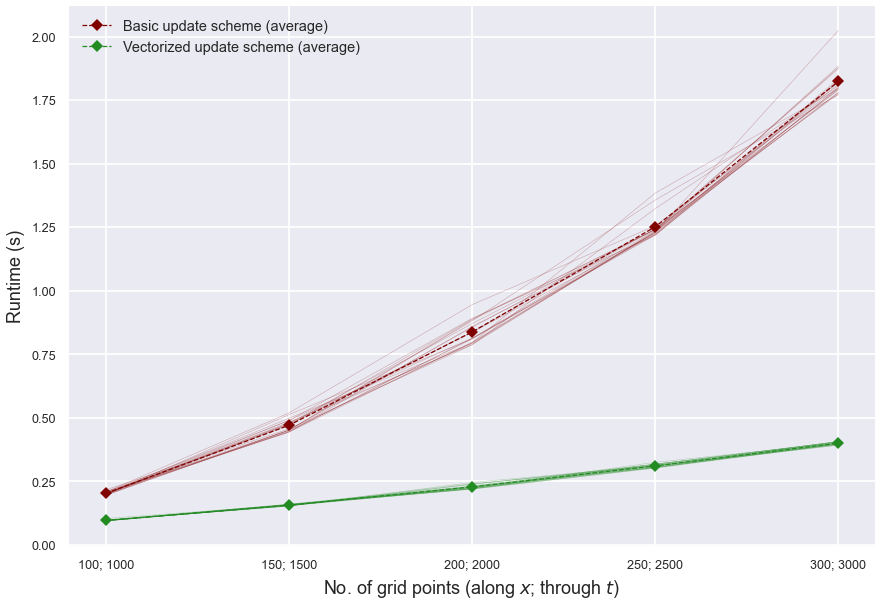
\includegraphics[scale=0.75]{on vectorization.png}
   % \includegraphics[scale=0.75]{runtimes-300.png}
   \caption{Execution times for basic and vectorized update schemes at different domain discretizations.}
	\label{fig: On Vectorization results}
\end{figure}

Runtimes for the different discretizations and update schemes are summarized in Fig. \ref{fig: On Vectorization results}.
The vectorized update scheme is significantly faster than the naive loop approach,
and the speedup gained increases as the domain discretization gets finer.
The disparity in the execution times is attributed to NumPy's support for array-based computing;
in fact, one can expect to arrive at similar findings when using other numerical computing tools such as
MATLAB\textsuperscript{\textregistered} \citep{MATLABR2020b}.
This suggests that, for the same computational resources and time duration,
vectorization enables one to iterate and model more scenarios
than using the explicit loop-based approach.

\subsection{On Spatial Domain Discretization}
\label{subsec: On Spatial Domain Discretization}

\lipsum[54]

\subsection{On Temporal Domain Discretization}
\label{subsec: On Temporal Domain Discretization}

\lipsum[92]

\subsection{A Multi-Stage Scenario}
\label{subsec: A Multi-Stage Scenario}

\lipsum[84]

\section{Conclusion}
\label{sec: Conclusion}

\lipsum[20]

%%---
\section*{Submission of conference papers to ICLR 2021}

ICLR requires electronic submissions, processed by
\url{https://openreview.net/}. See ICLR's website for more instructions.

If your paper is ultimately accepted, the statement {\tt
  {\textbackslash}iclrfinalcopy} should be inserted to adjust the
format to the camera ready requirements.

The format for the submissions is a variant of the NeurIPS format.
Please read carefully the instructions below, and follow them
faithfully.

\subsection*{Style}

Papers to be submitted to ICLR 2021 must be prepared according to the
instructions presented here.

%% Please note that we have introduced automatic line number generation
%% into the style file for \LaTeXe. This is to help reviewers
%% refer to specific lines of the paper when they make their comments. Please do
%% NOT refer to these line numbers in your paper as they will be removed from the
%% style file for the final version of accepted papers.

Authors are required to use the ICLR \LaTeX{} style files obtainable at the
ICLR website. Please make sure you use the current files and
not previous versions. Tweaking the style files may be grounds for rejection.

\subsection*{Retrieval of style files}

The style files for ICLR and other conference information are available online at:
\begin{center}
   \url{http://www.iclr.cc/}
\end{center}
The file \verb+iclr2021_conference.pdf+ contains these
instructions and illustrates the
various formatting requirements your ICLR paper must satisfy.
Submissions must be made using \LaTeX{} and the style files
\verb+iclr2021_conference.sty+ and \verb+iclr2021_conference.bst+ (to be used with \LaTeX{}2e). The file
\verb+iclr2021_conference.tex+ may be used as a ``shell'' for writing your paper. All you
have to do is replace the author, title, abstract, and text of the paper with
your own.

The formatting instructions contained in these style files are summarized in
sections \ref{gen_inst}, \ref{headings}, and \ref{others} below.

\section*{General formatting instructions}
\label{gen_inst}

The text must be confined within a rectangle 5.5~inches (33~picas) wide and
9~inches (54~picas) long. The left margin is 1.5~inch (9~picas).
Use 10~point type with a vertical spacing of 11~points. Times New Roman is the
preferred typeface throughout. Paragraphs are separated by 1/2~line space,
with no indentation.

Paper title is 17~point, in small caps and left-aligned.
All pages should start at 1~inch (6~picas) from the top of the page.

Authors' names are
set in boldface, and each name is placed above its corresponding
address. The lead author's name is to be listed first, and
the co-authors' names are set to follow. Authors sharing the
same address can be on the same line.

Please pay special attention to the instructions in section \ref{others}
regarding figures, tables, acknowledgments, and references.


There will be a strict upper limit of 8 pages for the main text of the initial submission, with unlimited additional pages for citations. Note that the upper page limit differs from last year!Authors may use as many pages of appendices (after the bibliography) as they wish, but reviewers are not required to read these. During the rebuttal phase and for the camera ready version, authors are allowed one additional page for the main text, for a strict upper limit of 9 pages.

\section*{Headings: first level}
\label{headings}

First level headings are in small caps,
flush left and in point size 12. One line space before the first level
heading and 1/2~line space after the first level heading.

\subsection*{Headings: second level}

Second level headings are in small caps,
flush left and in point size 10. One line space before the second level
heading and 1/2~line space after the second level heading.

\subsubsection*{Headings: third level}

Third level headings are in small caps,
flush left and in point size 10. One line space before the third level
heading and 1/2~line space after the third level heading.

\section*{Citations, figures, tables, references}
\label{others}

These instructions apply to everyone, regardless of the formatter being used.

\subsection*{Citations within the text}

Citations within the text should be based on the \texttt{natbib} package
and include the authors' last names and year (with the ``et~al.'' construct
for more than two authors). When the authors or the publication are
included in the sentence, the citation should not be in parenthesis using \verb|\citet{}| (as
in ``See \citet{Hinton06} for more information.''). Otherwise, the citation
should be in parenthesis using \verb|\citep{}| (as in ``Deep learning shows promise to make progress
towards AI~\citep{Bengio+chapter2007}.'').

The corresponding references are to be listed in alphabetical order of
authors, in the \textsc{References} section. As to the format of the
references themselves, any style is acceptable as long as it is used
consistently.

\subsection*{Footnotes}

Indicate footnotes with a number\footnote{Sample of the first footnote} in the
text. Place the footnotes at the bottom of the page on which they appear.
Precede the footnote with a horizontal rule of 2~inches
(12~picas).\footnote{Sample of the second footnote}

\subsection*{Figures}

All artwork must be neat, clean, and legible. Lines should be dark
enough for purposes of reproduction; art work should not be
hand-drawn. The figure number and caption always appear after the
figure. Place one line space before the figure caption, and one line
space after the figure. The figure caption is lower case (except for
first word and proper nouns); figures are numbered consecutively.

Make sure the figure caption does not get separated from the figure.
Leave sufficient space to avoid splitting the figure and figure caption.

You may use color figures.
However, it is best for the
figure captions and the paper body to make sense if the paper is printed
either in black/white or in color.
\begin{figure}[h]
\begin{center}
%\framebox[4.0in]{$\;$}
\fbox{\rule[-.5cm]{0cm}{4cm} \rule[-.5cm]{4cm}{0cm}}
\end{center}
\caption{Sample figure caption.}
\end{figure}

\subsection*{Tables}

All tables must be centered, neat, clean and legible. Do not use hand-drawn
tables. The table number and title always appear before the table. See
Table~\ref{sample-table}.

Place one line space before the table title, one line space after the table
title, and one line space after the table. The table title must be lower case
(except for first word and proper nouns); tables are numbered consecutively.

\begin{table}[t]
\caption{Sample table title}
\label{sample-table}
\begin{center}
\begin{tabular}{ll}
\multicolumn{1}{c}{\bf PART}  &\multicolumn{1}{c}{\bf DESCRIPTION}
\\ \hline \\
Dendrite         &Input terminal \\
Axon             &Output terminal \\
Soma             &Cell body (contains cell nucleus) \\
\end{tabular}
\end{center}
\end{table}

\section*{Default Notation}

In an attempt to encourage standardized notation, we have included the
notation file from the textbook, \textit{Deep Learning}
\cite{goodfellow2016deep} available at
\url{https://github.com/goodfeli/dlbook_notation/}.  Use of this style
is not required and can be disabled by commenting out
\texttt{math\_commands.tex}.


\centerline{\bf Numbers and Arrays}
\bgroup
\def\arraystretch{1.5}
\begin{tabular}{p{1in}p{3.25in}}
$\displaystyle a$ & A scalar (integer or real)\\
$\displaystyle \va$ & A vector\\
$\displaystyle \mA$ & A matrix\\
$\displaystyle \tA$ & A tensor\\
$\displaystyle \mI_n$ & Identity matrix with $n$ rows and $n$ columns\\
$\displaystyle \mI$ & Identity matrix with dimensionality implied by context\\
$\displaystyle \ve^{(i)}$ & Standard basis vector $[0,\dots,0,1,0,\dots,0]$ with a 1 at position $i$\\
$\displaystyle \text{diag}(\va)$ & A square, diagonal matrix with diagonal entries given by $\va$\\
$\displaystyle \ra$ & A scalar random variable\\
$\displaystyle \rva$ & A vector-valued random variable\\
$\displaystyle \rmA$ & A matrix-valued random variable\\
\end{tabular}
\egroup
\vspace{0.25cm}

\centerline{\bf Sets and Graphs}
\bgroup
\def\arraystretch{1.5}

\begin{tabular}{p{1.25in}p{3.25in}}
$\displaystyle \sA$ & A set\\
$\displaystyle \R$ & The set of real numbers \\
$\displaystyle \{0, 1\}$ & The set containing 0 and 1 \\
$\displaystyle \{0, 1, \dots, n \}$ & The set of all integers between $0$ and $n$\\
$\displaystyle [a, b]$ & The real interval including $a$ and $b$\\
$\displaystyle (a, b]$ & The real interval excluding $a$ but including $b$\\
$\displaystyle \sA \backslash \sB$ & Set subtraction, i.e., the set containing the elements of $\sA$ that are not in $\sB$\\
$\displaystyle \gG$ & A graph\\
$\displaystyle \parents_\gG(\ervx_i)$ & The parents of $\ervx_i$ in $\gG$
\end{tabular}
\vspace{0.25cm}


\centerline{\bf Indexing}
\bgroup
\def\arraystretch{1.5}

\begin{tabular}{p{1.25in}p{3.25in}}
$\displaystyle \eva_i$ & Element $i$ of vector $\va$, with indexing starting at 1 \\
$\displaystyle \eva_{-i}$ & All elements of vector $\va$ except for element $i$ \\
$\displaystyle \emA_{i,j}$ & Element $i, j$ of matrix $\mA$ \\
$\displaystyle \mA_{i, :}$ & Row $i$ of matrix $\mA$ \\
$\displaystyle \mA_{:, i}$ & Column $i$ of matrix $\mA$ \\
$\displaystyle \etA_{i, j, k}$ & Element $(i, j, k)$ of a 3-D tensor $\tA$\\
$\displaystyle \tA_{:, :, i}$ & 2-D slice of a 3-D tensor\\
$\displaystyle \erva_i$ & Element $i$ of the random vector $\rva$ \\
\end{tabular}
\egroup
\vspace{0.25cm}


\centerline{\bf Calculus}
\bgroup
\def\arraystretch{1.5}
\begin{tabular}{p{1.25in}p{3.25in}}
% NOTE: the [2ex] on the next line adds extra height to that row of the table.
% Without that command, the fraction on the first line is too tall and collides
% with the fraction on the second line.
$\displaystyle\frac{d y} {d x}$ & Derivative of $y$ with respect to $x$\\ [2ex]
$\displaystyle \frac{\partial y} {\partial x} $ & Partial derivative of $y$ with respect to $x$ \\
$\displaystyle \nabla_\vx y $ & Gradient of $y$ with respect to $\vx$ \\
$\displaystyle \nabla_\mX y $ & Matrix derivatives of $y$ with respect to $\mX$ \\
$\displaystyle \nabla_\tX y $ & Tensor containing derivatives of $y$ with respect to $\tX$ \\
$\displaystyle \frac{\partial f}{\partial \vx} $ & Jacobian matrix $\mJ \in \R^{m\times n}$ of $f: \R^n \rightarrow \R^m$\\
$\displaystyle \nabla_\vx^2 f(\vx)\text{ or }\mH( f)(\vx)$ & The Hessian matrix of $f$ at input point $\vx$\\
$\displaystyle \int f(\vx) d\vx $ & Definite integral over the entire domain of $\vx$ \\
$\displaystyle \int_\sS f(\vx) d\vx$ & Definite integral with respect to $\vx$ over the set $\sS$ \\
\end{tabular}
\egroup
\vspace{0.25cm}

\centerline{\bf Probability and Information Theory}
\bgroup
\def\arraystretch{1.5}
\begin{tabular}{p{1.25in}p{3.25in}}
$\displaystyle P(\ra)$ & A probability distribution over a discrete variable\\
$\displaystyle p(\ra)$ & A probability distribution over a continuous variable, or over
a variable whose type has not been specified\\
$\displaystyle \ra \sim P$ & Random variable $\ra$ has distribution $P$\\% so thing on left of \sim should always be a random variable, with name beginning with \r
$\displaystyle  \E_{\rx\sim P} [ f(x) ]\text{ or } \E f(x)$ & Expectation of $f(x)$ with respect to $P(\rx)$ \\
$\displaystyle \Var(f(x)) $ &  Variance of $f(x)$ under $P(\rx)$ \\
$\displaystyle \Cov(f(x),g(x)) $ & Covariance of $f(x)$ and $g(x)$ under $P(\rx)$\\
$\displaystyle H(\rx) $ & Shannon entropy of the random variable $\rx$\\
$\displaystyle \KL ( P \Vert Q ) $ & Kullback-Leibler divergence of P and Q \\
$\displaystyle \mathcal{N} ( \vx ; \vmu , \mSigma)$ & Gaussian distribution %
over $\vx$ with mean $\vmu$ and covariance $\mSigma$ \\
\end{tabular}
\egroup
\vspace{0.25cm}

\centerline{\bf Functions}
\bgroup
\def\arraystretch{1.5}
\begin{tabular}{p{1.25in}p{3.25in}}
$\displaystyle f: \sA \rightarrow \sB$ & The function $f$ with domain $\sA$ and range $\sB$\\
$\displaystyle f \circ g $ & Composition of the functions $f$ and $g$ \\
  $\displaystyle f(\vx ; \vtheta) $ & A function of $\vx$ parametrized by $\vtheta$.
  (Sometimes we write $f(\vx)$ and omit the argument $\vtheta$ to lighten notation) \\
$\displaystyle \log x$ & Natural logarithm of $x$ \\
$\displaystyle \sigma(x)$ & Logistic sigmoid, $\displaystyle \frac{1} {1 + \exp(-x)}$ \\
$\displaystyle \zeta(x)$ & Softplus, $\log(1 + \exp(x))$ \\
$\displaystyle || \vx ||_p $ & $\normlp$ norm of $\vx$ \\
$\displaystyle || \vx || $ & $\normltwo$ norm of $\vx$ \\
$\displaystyle x^+$ & Positive part of $x$, i.e., $\max(0,x)$\\
$\displaystyle \1_\mathrm{condition}$ & is 1 if the condition is true, 0 otherwise\\
\end{tabular}
\egroup
\vspace{0.25cm}



\section*{Final instructions}
Do not change any aspects of the formatting parameters in the style files.
In particular, do not modify the width or length of the rectangle the text
should fit into, and do not change font sizes (except perhaps in the
\textsc{References} section; see below). Please note that pages should be
numbered.

\section*{Preparing PostScript or PDF files}

Please prepare PostScript or PDF files with paper size ``US Letter'', and
not, for example, ``A4''. The -t
letter option on dvips will produce US Letter files.

Consider directly generating PDF files using \verb+pdflatex+
(especially if you are a MiKTeX user).
PDF figures must be substituted for EPS figures, however.

Otherwise, please generate your PostScript and PDF files with the following commands:
\begin{verbatim}
dvips mypaper.dvi -t letter -Ppdf -G0 -o mypaper.ps
ps2pdf mypaper.ps mypaper.pdf
\end{verbatim}

\subsection*{Margins in LaTeX}

Most of the margin problems come from figures positioned by hand using
\verb+\special+ or other commands. We suggest using the command
\verb+\includegraphics+
from the graphicx package. Always specify the figure width as a multiple of
the line width as in the example below using .eps graphics
\begin{verbatim}
   \usepackage[dvips]{graphicx} ...
   \includegraphics[width=0.8\linewidth]{myfile.eps}
\end{verbatim}
or % Apr 2009 addition
\begin{verbatim}
   \usepackage[pdftex]{graphicx} ...
   \includegraphics[width=0.8\linewidth]{myfile.pdf}
\end{verbatim}
for .pdf graphics.
See section~4.4 in the graphics bundle documentation (\url{http://www.ctan.org/tex-archive/macros/latex/required/graphics/grfguide.ps})

A number of width problems arise when LaTeX cannot properly hyphenate a
line. Please give LaTeX hyphenation hints using the \verb+\-+ command.


%\subsubsection*{Author Contributions}
%If you'd like to, you may include  a section for author contributions as is done
%in many journals. This is optional and at the discretion of the authors.

%\subsubsection*{Acknowledgments}
%Use unnumbered third level headings for the acknowledgments. All
%acknowledgments, including those to funding agencies, go at the end of the paper.

%\bibliography{iclr2021_conference}
\bibliography{references}
\bibliographystyle{iclr2021_conference}

%\appendix
%\section{Appendix}
%You may include other additional sections here.

\end{document}
